\documentclass[11pt]{amsart}
\usepackage{booktabs}
\usepackage{amsmath,amssymb,graphicx,lmodern}
\usepackage[hidelinks]{hyperref}
\hypersetup{pdftitle={Sperner's Lemma and Fixed Points of Multivalued Maps on Cubes},pdfauthor={Yitzchak Shmalo}}
\newtheorem{thm}{Theorem}[section]
\newtheorem{lem}[thm]{Lemma}
\newtheorem{cor}[thm]{Corollary}
\newtheorem{prop}[thm]{Proposition}
\theoremstyle{definition}
\newtheorem{defn}[thm]{Definition}
\newtheorem{ex}[thm]{Example}
\theoremstyle{remark}
\newtheorem{rem}[thm]{Remark}
\numberwithin{equation}{section}
\newcommand{\R}{\mathbb R}
\DeclareMathOperator{\conv}{conv}
\DeclareMathOperator{\car}{car}
\addtolength{\hoffset}{-0.8cm}
\addtolength{\textwidth}{1.8cm}

\title[Sperner's lemma and multivalued fixed points]{Sperner's Lemma and Fixed Points of Multivalued Maps on Cubes}
\author[Yitzchak Shmalo]{Yitzchak Shmalo}
\address{Einstein Institute of Mathematics, The Hebrew University of Jerusalem, Jerusalem, Israel}
\email{yitzchak.shmalo@gmail.com}
\subjclass[2020]{Primary 47H10; Secondary 54H25, 52B05}
\keywords{Fixed points, Sperner's lemma, cubical complex, Brouwer, Kakutani}

\begin{document}
\begin{abstract}
For an upper semicontinuous map $f$ of the cube $[-1,1]^d$ with nonempty compact convex values, label the vertices of a cubical subdivision by the coordinate signs of $y_v-v$, where $y_v\in f(v)$, with the inward sign at a zero coordinate on the boundary. Some cube then carries all $2^d$ labels or has a facet whose labels are not the corners of the cube on one side of a hyperplane, and along a subsequence of subdivisions of vanishing mesh some sequence of such cubes, or of such facets, shrinks to a fixed point of $f$. No Lipschitz bound is assumed. The existence of such a cube follows from a Sperner lemma for cells labeled by the vertices of a polytope, which holds when the piecewise affine map determined by the labels has nonzero degree on the boundary and the labels of each facet satisfy a condition. Kakutani's interpolation argument, with Sperner's lemma in place of Brouwer's theorem, gives on a cube Kakutani's theorem and a fixed point theorem of Bich for maps that need not be upper semicontinuous.
\end{abstract}
\maketitle

\section{Introduction}\label{sec:intro}
A cubical subdivision of the cube $C=[-1,1]^d$ is a subdivision of $C$ into $d$-dimensional cubes meeting face to face, and the mesh of a subdivision is the largest diameter of a cell. When a point $y_v$ is chosen at each vertex $v$, its displacement is $u_v=y_v-v$.

Gidea and Shmalo \cite{GS1} label the vertices of a cubical subdivision of $C$ by vectors in $\{-1,1\}^d$. If the labeling is non-degenerate, that is, no face of $\partial C$ carries $d+1$ labels in which every coordinate takes both signs, and its oriented index, a signed count of faces \cite[\S2.2]{GS1}, is nonzero, some cube carries $d+1$ labels in which every coordinate takes both signs \cite[Theorem~3.4]{GS1}. When the labels are the coordinate signs of the displacements of a map, the points of such a cube are approximate fixed points, for planar maps under Lipschitz bounds \cite[Proposition~4.6]{GS1} and for bi-Lipschitz maps in any dimension once the subdivision is fine \cite[Proposition~4.10]{GS1}. For upper semicontinuous multivalued maps this fails at every mesh below $1/20$, as the example below shows.

Let $f$ assign to each point of $C$ a nonempty compact convex subset of $C$, upper semicontinuously. At each vertex $v$ of a cubical subdivision choose $y_v\in f(v)$ and label $v$ by a sign label of $u_v$, that is, a vector $s_v\in\{-1,1\}^d$ with $s_{v,j}u_{v,j}\ge0$ for every $j$; on a zero coordinate take the inward sign $s_{v,j}=-v_j$ when $v_j=\pm1$, and either sign otherwise. We call this the \emph{sign rule}. The labels are corners of $C$. A facet of a cube of the subdivision is \emph{problematic} if its labels do not form an affine cut set, that is, are not the corners on one side of a hyperplane that misses every corner and has corners on both sides (Section~\ref{cubicle}).

For $d=2$, let $K$ be the triangle with vertices $(1/2,1/2)$, $(-3/5,1/2)$ and $(1/2,-3/5)$, and let $f(x)=K$ for every $x$, so that the fixed points of $f$ are the points of $K$. Take a square of the subdivision with side less than $1/20$ that contains $(-1/2,-1/2)$, and choose the images $(1/2,1/2)$ at two of its vertices and $(-3/5,1/2)$ and $(1/2,-3/5)$ at the other two. Each displacement is within $1/20$ in each coordinate of $(1,1)$, $(1,1)$, $(-1/10,1)$ or $(1,-1/10)$. The labels of the square therefore contain three vectors with both signs in every coordinate, yet every displacement has positive dot product with $(1,1)$, so $0$ is not in the convex hull of the displacements. Every point of the square has distance more than $1/2$ from $K$.

\begin{thm}[Theorem~\ref{4.4}]\label{thm:intro}
Let $f$ assign to each point of $C$ a nonempty compact convex subset of $C$, upper semicontinuously. For each $m$ let $\mathcal Q_m$ be a cubical subdivision of $C$ with mesh $h_m\to0$, labeled by the sign rule with images $y_v\in f(v)$. There exist $m_k\to\infty$, a point $x\in f(x)$ and sets $F_k$ with $\sup_{z\in F_k}\|z-x\|\to0$, where either every $F_k$ is a cube of $\mathcal Q_{m_k}$ whose vertices carry all $2^d$ sign labels, or every $F_k$ is a problematic facet of a cube of $\mathcal Q_{m_k}$.
\end{thm}

Cubes whose vertices carry all $2^d$ sign labels accumulate only at fixed points of $f$ (Proposition~\ref{prop:cubehull}). Problematic facets need not: for $d=3$ and the constant map with value $\{y\in C:y_1=1\}$, the images can be chosen so that at every mesh below $1/2$ some problematic facet has distance at least $1$ from every fixed point (Remark~\ref{rem:farfacet}). For them Theorem~\ref{thm:intro} gives one sequence that shrinks to a fixed point. The proof finds, at a vertex $v$ of a cube of one of these two kinds, a convex combination $n=\sum_w\lambda_wu_w$ of displacements at vertices $w$ of cubes containing $v$ that lies in the normal cone $N_C(v)=\{n:n\cdot(z-v)\le0\text{ for all }z\in C\}$. If there were none, vectors $a_v$ separating these displacements from $N_C(v)$, combined with the affine interpolation of the sign labels, would give a vector field on $C$ without zeros that points strictly inward on $\partial C$. Brouwer's theorem excludes such a field. With $\bar v=\sum_w\lambda_ww$ and $q=\sum_w\lambda_wy_w$ one has $q-\bar v=n$ and $n\cdot(q-v)\le0$, so that
\begin{equation}\label{intro:est}
\|q-v\|^2+\|n\|^2\le\|\bar v-v\|^2\le h^2,
\end{equation}
where $h$ is the mesh. Thus a convex combination of chosen images lies within $h$ of $v$, and no Lipschitz bound and no non-degeneracy assumption enters. A cube carrying all $2^d$ sign labels already has $0$ in the convex hull of its displacements (Proposition~\ref{prop:cubehull}), and cells with this property can be selected from the displacements themselves, as for the vector labelings of Eaves \cite{Eaves} and van der Laan \cite[\S4.8]{Laa80} (Propositions~\ref{prop:balance} and~\ref{prop:limit} below). Theorem~\ref{4.4} uses only the signs of the coordinates of the displacements, which is all that the labels of \cite{GS1} record. By Corollary~\ref{cor:marked}, every labeling by the sign rule has a cube whose vertices carry all $2^d$ sign labels or a problematic facet.

The existence of such a cube or facet is a case of a Sperner lemma for labels at the vertices of a polytope. Let a subdivision of a convex $d$-polytope $P$ be labeled by the vertices of a convex $d$-polytope $P'$, its corners (Section~\ref{cubicle}), as in Definition~\ref{facetdata}: labels sit at the vertices of the subdivision and possibly at points inside facets of cells, a cell is completely labeled if it carries every corner, and the boundary degree is the degree on $\partial P$ of the affine interpolation $S$ of the vertex labels. A nonzero boundary degree does not give a completely labeled cell, even when the labels carried by each facet form an affine cut set: in Example~\ref{ex:sixtet} six tetrahedra subdivide $[0,1]^3$, the boundary degree is one, and every tetrahedron misses a corner. By Theorem~\ref{thm:YS3} some cell is completely labeled if the boundary degree is nonzero and one point $p$ in the interior of $P'$ satisfies
\begin{equation}\label{intro:ray}
\conv A_D\cap[p,\ell]=\varnothing\qquad\text{for every facet $D$ with $A_D\ne V$ and every $\ell\in V\setminus A_D$}.
\end{equation}
Here $V$ is the set of corners, $A_D$ the set of labels carried by $D$, $\conv$ the convex hull and $[p,\ell]$ the segment from $p$ to $\ell$. In Example~\ref{ex:sixtet} no point $p$ satisfies \eqref{intro:ray}, and in Example~\ref{ex:hexagon} it fails on a single facet. Condition \eqref{intro:ray} holds when a hyperplane strictly separates $A_D$ from $\{p\}\cup(V\setminus A_D)$, and when $A_D$ lies in a proper face of $P'$ (Corollary~\ref{cor:YS3}). On a cubical subdivision of a cube labeled only at its vertices by the corners of $[-1,1]^d$, if the labels of each facet form an affine cut set, then the center satisfies \eqref{intro:ray} (Lemma~\ref{lem:cut}).

When the labels are the $d+1$ vertices of a simplex, Bekker and Netsvetaev \cite{Bekker1995} introduced an index of the labeling, a recursive count over faces taken modulo two \cite[Remark~2.2]{GS1}. Gidea and Shmalo \cite[\S2.2]{GS1} count the same faces with orientation signs, which gives the oriented index. If no facet of $P$ carries all $d+1$ labels, the oriented index equals, up to sign, the degree of the restriction to $\partial P$ of any continuous map of $P$ that sends each vertex to its label and each face into the convex hull of its labels. If it is nonzero, some cell carries all $d+1$ labels (Bekker and Netsvetaev \cite{Bekker1995}; see \cite[Proposition~2.4 and Theorem~2.6]{GS1} for the oriented form). When $P'$ is a simplex, every proper set of labels lies in a proper face, so \eqref{intro:ray} holds by Corollary~\ref{cor:YS3}(b) and the only hypothesis left in Theorem~\ref{thm:YS3} is nonzero boundary degree. For a simplex this gives the theorem of Bekker and Netsvetaev in the oriented form of \cite[Theorem~2.6]{GS1}, with the boundary degree in place of the oriented index.

Labelings by the vertices of a polytope have been studied mainly on triangulations. De Loera, Peterson and Su \cite{DLPS02} proved a conjecture of Atanassov: if a triangulation of a $d$-polytope with $k$ vertices is labeled so that a vertex in the relative interior of a face $F$ receives the label of a vertex of $F$, then at least $k-d$ full-dimensional simplices carry $d+1$ distinct labels. Meunier \cite{Meu06} extended this theorem to piecewise linear $d$-manifolds with boundary embedded in $\mathbb{R}^d$, and Musin \cite{Musin15} gave further extensions to manifolds, proved with the degree of the piecewise linear map determined by the labels. In these results the cells are simplices, so a cell carries at most $d+1$ labels, whereas Theorem~\ref{thm:YS3} allows cells that are arbitrary polytopes and asks for a cell carrying every corner of $P'$. On cubes, the cubical Sperner lemma of Ky Fan~\cite{Fan60}, in the form stated by Meunier \cite[Theorem~5]{Meu08}, labels a cubical subdivision of a cube by its corners so that each label is a corner of the smallest face containing its vertex and adjacent vertices receive equal or adjacent corners. Some small cube then has its vertices mapped bijectively onto the corners. In place of this adjacency requirement, Theorem~\ref{thm:YS3} assumes nonzero boundary degree and \eqref{intro:ray}. Other cubical forms of Sperner's lemma are due to Kuhn \cite{Kuhn60}, who labels each point of the grid $\{0,\ldots,k\}^d$ by a vertex of $\{0,1\}^d$ whose $i$th coordinate is $0$ when $x_i=0$ and $1$ when $x_i=k$, and finds grid points $v_0<v_1<\cdots<v_d\le v_0+(1,\ldots,1)$ on which every coordinate of the labels takes both values, to Wolsey \cite{Wol77}, who derived them from generalized complementary pivoting, and to Freund \cite{Fre84}, who proved two dual combinatorial lemmas on the cube by path following on variable dimension complexes.

By Theorem~\ref{thm:YS3} with $p=0$, every cubical subdivision of $C$ labeled by the sign rule contains a completely labeled cube or a problematic facet (Corollary~\ref{cor:marked}). Theorem~3.4 of \cite{GS1} assumes a non-degenerate labeling with nonzero oriented index; Corollary~\ref{cor:marked} assumes only the sign rule, which gives boundary degree $(-1)^d$. Since only vertices carry labels here, a completely labeled cube is one whose vertices carry all $2^d$ sign labels. For a single cube, neither the conclusion of Corollary~\ref{cor:marked} nor that of \cite[Theorem~3.4]{GS1} implies the other. For $d=3$, let all labels of a cube have first coordinate $1$ and let one of its facets carry exactly the labels $(1,1,1)$ and $(1,-1,-1)$. These two corners are not an affine cut set, since the two diagonals of the square of corners with first coordinate $1$ cross, so the facet is problematic, yet no label has first coordinate $-1$. In the square with displacements $(1,1)$, $(1,1)$, $(-1/10,1)$ and $(1,-1/10)$ above, put the two displacements $(1,1)$ at opposite vertices. Every edge then carries two adjacent corners, which form an affine cut set, and the square carries three of the four sign labels, and these three take both signs in every coordinate.

Kakutani's theorem states that if $f$ assigns to each point of a simplex a nonempty compact convex subset of the simplex and is upper semicontinuous, then $x\in f(x)$ for some point $x$ \cite[Theorem~1]{KF}. Multivalued maps of this kind are used to approximate single-valued maps in computations \cite{Kaczynski2008}, and Mischaikow and Mrozek \cite{MM} use them to study the Lorenz equations. Kakutani \cite{KF} chose one image $y_v\in f(v)$ at each vertex $v$ of a triangulation, interpolated these choices affinely on each simplex, and applied Brouwer's theorem to this interpolant. As the mesh of the triangulation tends to zero, a subsequence of the fixed points of the interpolants converges to a fixed point of $f$. Several later proofs use Sperner's lemma in place of Brouwer's theorem. Sondjaja \cite[\S3.3]{LM} builds a Sperner labeling from von Neumann's continuous approximations to the graph of $f$. Le, Le Van, Pham and Sa\u{g}lam \cite[\S3.3, Theorem~1]{Le} use a covering argument. Tanaka \cite{YT} proves a constructive approximate form, and Eaves \cite{Eaves} gives an algorithm that generates a sequence whose accumulation points are fixed points; it is one of the first methods that search for a simplex on which the affine interpolation of the chosen images has a fixed point. The argument with which Knaster, Kuratowski and Mazurkiewicz \cite{KKM29} derive Brouwer's theorem from Sperner's lemma gives an exact fixed point of a piecewise affine map, with no passage to a limit (Lemma~\ref{pl}). Applied to this interpolant, it gives Proposition~\ref{prop:balance}. For every finite subdivision of $C$ into convex polytopes meeting face to face and every choice of a point $y_v\in C$ at each vertex $v$, some cell $Q$ satisfies
\begin{equation}\label{intro:hull}
     0\in\conv\{\,y_v-v : v\text{ is a vertex of }Q\,\}.
\end{equation}
For a simplex $Q$, condition \eqref{intro:hull} holds exactly when the affine interpolation of the points $y_v$ has a fixed point in $Q$, which is the condition that the vector labeling of van der Laan places on a simplex \cite[\S4.8]{Laa80}. The points $y_v$ are arbitrary. If $y_v\in f(v)$, cells satisfying \eqref{intro:hull} on subdivisions of vanishing mesh accumulate only at fixed points of $f$ (Proposition~\ref{prop:limit}), which gives Kakutani's theorem on a cube (Theorem~\ref{5}).

Because the choices are arbitrary, the same step gives fixed points of maps that are not upper semicontinuous. Suppose $f$ has nonempty values and each point $x\notin f(x)$ has a relative neighborhood $U$ and a nonzero vector $a$ with $a\cdot(y-z)>0$ for all $z\in U$ with $z\notin f(z)$ and all $y\in f(z)$. If $f$ had no fixed point, then $a\cdot(y_v-v)>0$ at every vertex of a cell inside $U$, and no such cell would satisfy \eqref{intro:hull}. Hence $f$ has a fixed point (Theorem~\ref{extensions}). This is the case of a cube of a theorem of Bich \cite[Theorem~3.2]{Bich06}, which holds on any compact convex subset of a Banach space. Upper semicontinuous maps with nonempty compact convex values satisfy the hypothesis (Proposition~\ref{prop:usc-sep}), and the same selection of cells gives, on a cube, the theorem of Herings, van der Laan, Talman and Yang~\cite{HLTY} on locally gross direction preserving maps, those whose displacements near each nonfixed point have pairwise nonnegative dot products (Corollary~\ref{cor:hlty}).

Section~\ref{cubicle} proves Theorem~\ref{thm:YS3}. Section~\ref{kakutani} selects cells satisfying \eqref{intro:hull} and reproves Kakutani's theorem on a cube, Section~\ref{sec:sign} proves Theorem~\ref{4.4}, and Section~\ref{sec:sep} reproves, on a cube, the theorems of Bich and of Herings, van der Laan, Talman and Yang for maps that are not upper semicontinuous.

\section{Preliminaries}\label{pre}
\begin{defn}[Sperner labeling]
Consider the standard $d$-dimensional simplex $T=\conv(0,e_1,\ldots,e_d)\subset\R^d$, where $(e_1,\ldots,e_d)$ is the standard basis. A triangulation of $T$ is a finite subdivision into simplices such that the intersection of any two simplices is either empty or a face of both. If $K$ is a subset of $T$, the carrier $\car(K)$ is the smallest face of $T$ that contains $K$.

A Sperner labeling of the triangulation assigns to each vertex $v$ a number $\phi(v)\in\{0,\ldots,d\}$ such that
\begin{itemize}
\item[(i)] the vertices of $T$ have distinct labels,
\item[(ii)] each triangulation vertex $v$ is assigned one of the labels of the vertices of $T$ in $\car(\{v\})$.
\end{itemize}
\end{defn}

\begin{thm}[Sperner's lemma {\cite{Sperner1928}}]\label{sperner}
Every triangulation of $T$ with a Sperner labeling contains an odd number of $d$-simplices whose vertices carry all $d+1$ labels.
\end{thm}
In Figure~\ref{fig:sperner} exactly one triangle carries all three labels.

\begin{figure}[ht]
\centering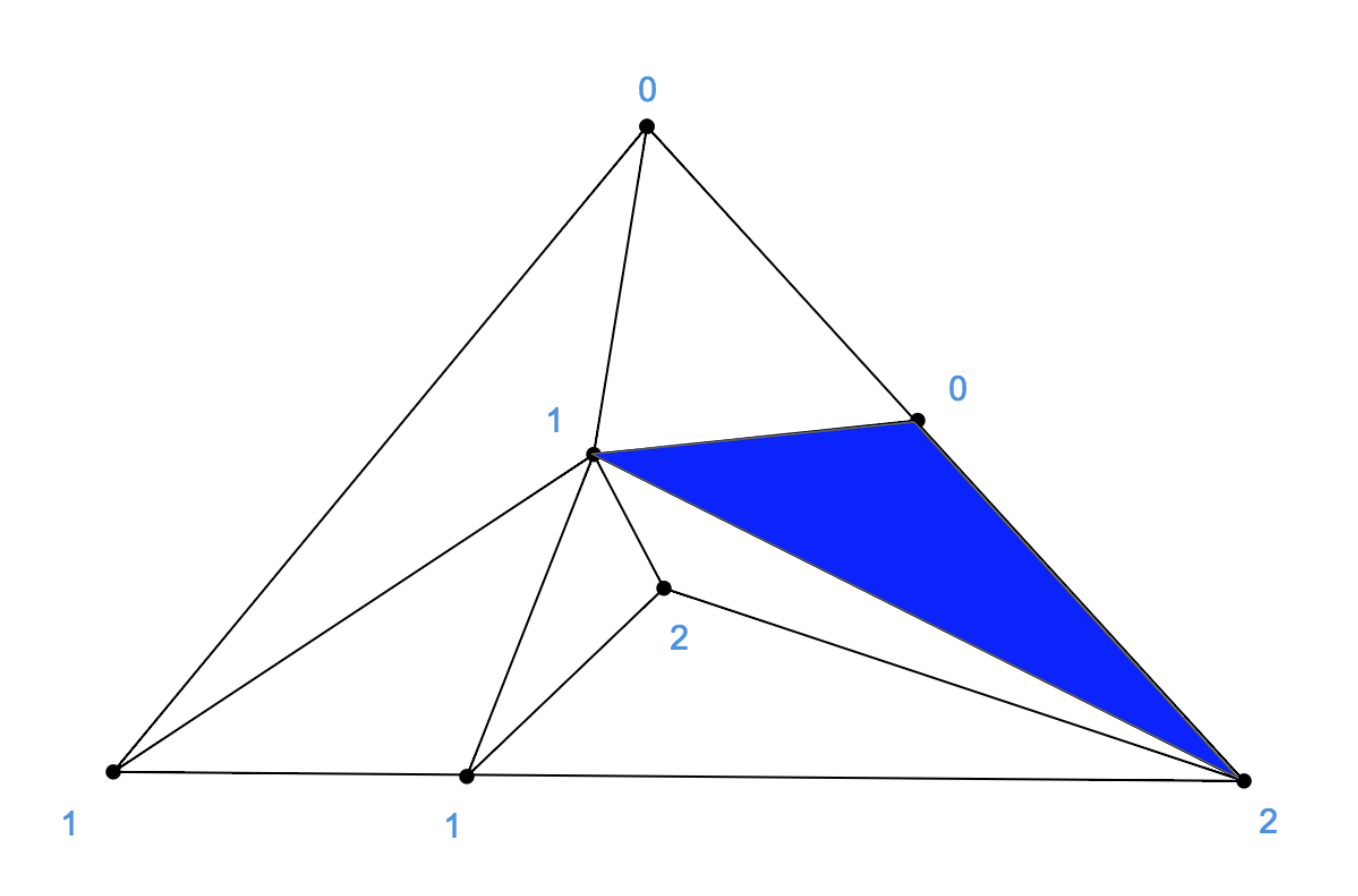
\includegraphics[width=.49\textwidth]{Sperner.png}
\caption{A Sperner labeling of a triangle. The shaded triangle carries all three labels.}\label{fig:sperner}
\end{figure}

\begin{thm}[Brouwer's fixed point theorem {\cite{Brou11}, \cite[Theorem~1.12.6]{BurnsG2005}}]\label{brouwer}
Let $T$ be a $d$-dimensional simplex and $F:T\to T$ be a continuous function. Then there exists a point $x\in T$ such that $F(x)=x$.
\end{thm}

Write $U_\delta(A)$ for the open $\delta$-neighborhood of a set $A$, relative to the space under consideration, and $U_\delta(x)$ for $U_\delta(\{x\})$.
\begin{defn}
A multivalued map $f:X\to 2^Y$ between metric spaces with nonempty compact values is upper semicontinuous if, for every $x\in X$ and every $\epsilon>0$, there exists a $\delta>0$ such that $f(z)\subset U_\epsilon(f(x))$ whenever $z\in U_\delta(x)$.
\end{defn}
In particular, if $x_j\to x$, $y_j\in f(x_j)$ and $y_j\to y$, then $\operatorname{dist}(y_j,f(x))\to0$. Since $f(x)$ is closed, $y\in f(x)$.

\begin{thm}[Kakutani's fixed point theorem on a simplex {\cite[Theorem~1]{KF}}]\label{kaksimplex}
Let $T$ be a $d$-dimensional simplex and let $f$ be an upper semicontinuous multivalued map from $T$ to nonempty, convex and compact subsets of $T$. Then there exists a point $x\in T$ such that $x\in f(x)$.
\end{thm}

Lemma~\ref{pl} is a consequence of Theorem~\ref{brouwer}; it also follows from Theorem~\ref{sperner} alone. Proposition~\ref{prop:balance} and Theorem~\ref{5} use Lemma~\ref{pl} and do not use Theorem~\ref{brouwer}.
\begin{lem}\label{pl}
Let $g$ be a continuous self-map of a simplex or a cube that is affine on each of finitely many convex polytopes covering it (its regions of affinity; such a map is called piecewise affine). Then $g$ has a fixed point.
\end{lem}
\begin{proof}
First let $g$ map a simplex $T$ into itself, and write $\beta_i(x)$ for the barycentric coordinate of $x$ at its $i$th vertex, $0\le i\le d$. The differences
\[
            r_i(x)=\beta_i(x)-\beta_i(g(x))
            \qquad (0\le i\le d)
\]
sum to zero. In each region of affinity, cut along the zero hyperplanes of the nonconstant $r_i$. Extend the bounding and cutting hyperplanes across $T$ and triangulate the resulting polytopes by barycentric subdivision. Each $r_i$ is nonnegative on the whole of each simplex or nonpositive on the whole of it.

Suppose $g(w)\ne w$ at every subdivision vertex $w$. Some $r_i(w)$ is positive, since the differences sum to zero and cannot all vanish at $w$. Give $w$ one such label $i$; the argument follows the derivation of Brouwer's theorem from Sperner's lemma by Knaster, Kuratowski and Mazurkiewicz \cite{KKM29}. Then $\beta_i(w)>0$, so the label belongs to its carrier. By Theorem~\ref{sperner} some simplex carries all $d+1$ labels. Each $r_i$ is positive at its labeled vertex and hence nonnegative throughout this simplex. Their sum is zero, which forces every $r_i$ to vanish there. This contradicts the strict inequality at the labeled vertices.

For a cube, choose coordinates in which $C=[-1,1]^d$, enclose it in a simplex $T$, and let $\rho:\R^d\to C$ clamp each coordinate to $[-1,1]$. If $g:C\to C$, apply the simplex argument to $\tilde g=g\circ\rho$. To obtain its regions of affinity, first cut along the hyperplanes $x_j=\pm1$, then pull back the regions of affinity of $g$ on each piece where $\rho$ is affine. The simplex argument gives a vertex $x$ with $\tilde g(x)=x$. Since $\tilde g$ takes values in $C$, $x\in C$ and $\rho(x)=x$. Thus $g(x)=x$.
\end{proof}

\section{Sperner's lemma with a boundary degree}\label{cubicle}
All subdivisions are finite, and their cells are convex polytopes meeting face to face. Let $P'$ be a convex $d$-polytope with vertex set $V$, whose elements we call corners. A set of corners is an \emph{affine cut set} if it consists of the corners in one open half-space of a hyperplane that misses every corner and has corners on both sides. For the unit cube $[0,1]^3$, with corners written as binary strings $x_1x_2x_3$, the four corners with $x_3=0$ form an affine cut set, and so do the four with $x_3=1$ (Figure~\ref{fig:crosssectionofcubes}).
\begin{figure}[ht]
\centering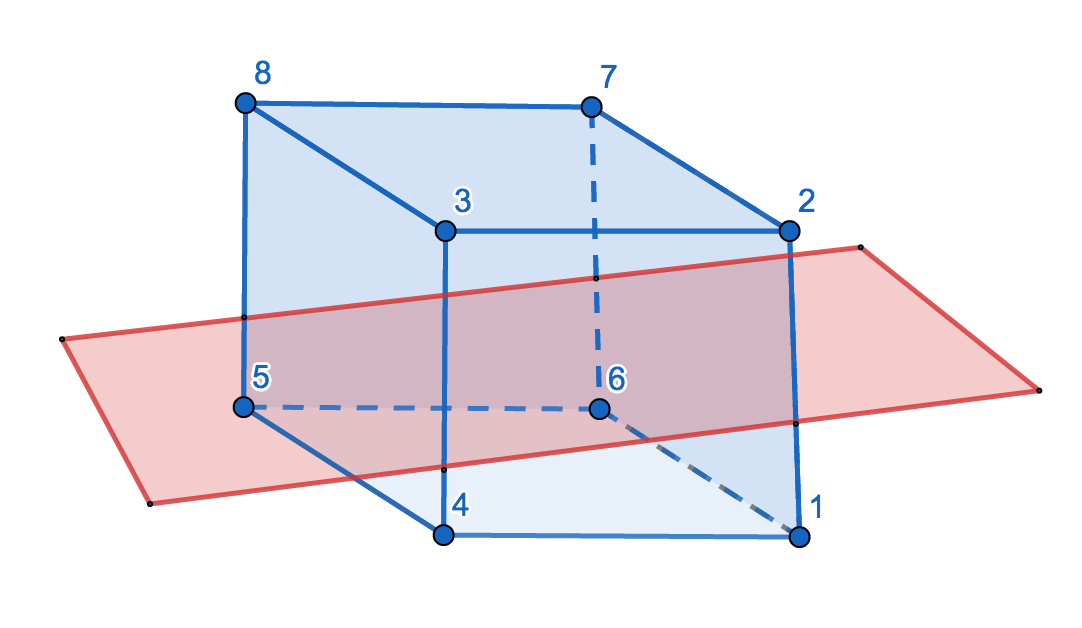
\includegraphics[width=.48\textwidth]{crosssectioncube.png}
\caption{A plane separating the four corners with $x_3=0$ (numbered $4,1,6,5$ for $000,100,110,010$) from the four with $x_3=1$ (numbered $3,2,7,8$ for $001,101,111,011$).}\label{fig:crosssectionofcubes}
\end{figure}

An \emph{orthant cut set} is the set of corners of a nonempty proper face of the cube $[-1,1]^d$, or the complement of such a set. Both are affine cut sets because the sum of the prescribed signed coordinates attains its maximum precisely on the face. Three corners of a square face in dimension three form an affine cut set, whereas an orthant cut set there has size $1,2,4,6$ or $7$.

To triangulate a subdivision without new vertices, order its vertices once and triangulate each cell by coning from its least vertex over the triangulations of the facets that omit that vertex. The construction restricts to the same triangulation on shared faces and introduces no vertices.

\begin{defn}[Labeling of a subdivision]\label{facetdata}
Let $P$ and $P'$ be convex $d$-polytopes, $d\ge1$. Label each vertex of a subdivision of $P$ into cells $Q_i$ by a corner of $P'$. Each facet $D$ of a cell may also carry finitely many labeled points in its relative interior. Both incident cells use the same data on a shared facet. Let $A_D$ consist of all labels on $D$. In dimension one a facet is a single vertex, and extra labels may be attached at that vertex. Choose a triangulation that refines the subdivision using only subdivision vertices. Let $S$ be affine on each simplex, taking at each subdivision vertex its label. The added labels do not prescribe values of $S$. A cell carries its vertex labels and all labels on its facets, and it is completely labeled if it carries every element of $V$. When $S(\partial P)\subset\partial P'$, the degree of $S|_{\partial P}\colon\partial P\to\partial P'$ is the \emph{boundary degree}. We orient the polytopes in their affine spans and their boundaries by the induced orientations. In dimension one we use reduced degree on the two boundary points. For the degree and its homotopy invariance see \cite[\S7.2]{BurnsG2005}.
\end{defn}

\begin{thm}[Sperner's lemma with a boundary degree]\label{thm:YS3}
Let a subdivision of a convex $d$-polytope $P$ be labeled by the corners of $P'$ as in Definition~\ref{facetdata}, with interpolation $S$ and facet label sets $A_D$. Suppose $S(\partial P)\subset\partial P'$, $\deg(S|_{\partial P})\ne0$, and there is a point $p\in\operatorname{int}P'$ such that $\conv A_D\cap[p,\ell]=\varnothing$ for every facet $D$ with $A_D\ne V$ and every $\ell\in V\setminus A_D$. Then some cell $Q_i$ is completely labeled.
\end{thm}

\begin{proof}
If some facet carries every label, any incident cell is completely labeled. Otherwise consider a cell $Q$ missing a label $\ell\in V$. For each facet $D$ of $Q$, $S(D)\subset\conv A_D$ and $\ell\notin A_D$, so $S(D)$ misses $[p,\ell]$. Since $p$ is interior and the corner $\ell$ is an extreme point of $P'$, the ray from $p$ through $\ell$ meets $P'$ precisely in $[p,\ell]$. It follows that
\[
x\longmapsto \frac{S(x)-p}{\|S(x)-p\|},\qquad x\in\partial Q,
\]
misses the unit direction $\eta=(\ell-p)/\|\ell-p\|$. It extends to a sphere-valued map on $Q$. Indeed, on each segment from a boundary point to a fixed interior point of $Q$ interpolate its boundary value linearly to $-\eta$ and normalize. Such a segment of values could pass through zero only if its initial value were $\eta$. The extensions from all cells that are not completely labeled agree on their boundaries, where they equal the displayed map.

If no cell were completely labeled, gluing the extensions would give a sphere-valued map on $P$ with the prescribed boundary values. Its boundary degree would be zero, since contracting $P$ to a point contracts its restriction as a sphere-valued map. Radial projection from $p$ is a homeomorphism from $\partial P'$ to the unit sphere. Composing with it preserves nonvanishing of the degree, contrary to the assumption on $S$.
\end{proof}

\begin{cor}\label{cor:YS3}
The hypothesis of Theorem~\ref{thm:YS3} on $p$ holds in each of the following cases.
\begin{enumerate}
\item[(a)] For each facet $D$ with $A_D\ne V$ an affine hyperplane strictly separates $A_D$ from $\{p\}\cup(V\setminus A_D)$.
\item[(b)] For each facet $D$ with $A_D\ne V$ the labels $A_D$ lie in one proper face of $P'$, which may depend on $D$; here $p$ is any interior point.
\end{enumerate}
\end{cor}

\begin{proof}
In (a), $p$ and $\ell$ lie in the open half-space not containing $\conv A_D$, and so does $[p,\ell]$. In (b), $\conv A_D$ lies in a proper face, hence in $\partial P'$. Every point of $[p,\ell)$ is interior to $P'$, and $\ell\notin\conv A_D$ because $\ell$ is a corner not in $A_D$.
\end{proof}

When $P=P'$ and the label at each vertex $v$ belongs to the carrier of $v$, defined as in Section~\ref{pre} with $P$ in place of $T$, $S$ maps each boundary face into itself. The straight homotopy to the identity stays in each such face, so the boundary degree is one.

\begin{ex}[A cube with no completely labeled tetrahedron]\label{ex:sixtet}
This subdivision of the cube has boundary degree one and every $A_D$ an affine cut set, yet each of its six tetrahedra misses a label and no point $p$ satisfies the hypothesis of Theorem~\ref{thm:YS3}. There are two labelings, one in which every $A_D$ is an affine cut set and one in which every $A_D$ is an orthant cut set. The labels at interior points of facets are needed: by Lemma~\ref{lem:cut}, applied in the coordinates $2x-(1,1,1)$, if every facet carried at most four labels forming an affine cut set, the center of the cube would satisfy the hypothesis of Theorem~\ref{thm:YS3}.

Let $P=P'=[0,1]^3$, with each corner labeled by itself. Write $v_{-}=000$, $v_{+}=111$ and, in cyclic order,
\[
(v_0,v_1,v_2,v_3,v_4,v_5)=(100,110,010,011,001,101),
\]
with indices read modulo six. The tetrahedra $Q_i=\conv(v_{-},v_{+},v_i,v_{i+1})$ are the six regions obtained by putting the three coordinates in all possible orders; for example $Q_0$ is $1\ge x_1\ge x_2\ge x_3\ge0$, and the successive differences of the coordinates are its barycentric weights. Equalities between adjacent coordinates give the common triangles $D_i=\conv(v_{-},v_{+},v_i)$.

In both labelings each $D_i$ carries a distinct point in its relative interior for each label needed to give precisely
\[
                     A_{D_i}=V\setminus\{v_{i+2},v_{i+3}\}.
\]
The two omitted labels form an edge. Under the change to sign coordinates $x\mapsto2x-(1,1,1)$, the sum of the two signed coordinates fixed on that edge is $2$ there and at most $0$ elsewhere. Thus the complement of $A_{D_i}$ is an affine cut set, and it is also an orthant cut set, since the excluded edge is a face of the cube; so $A_{D_i}$ is a cut set of both kinds. Without the added points the label set of $D_i$ is $\{v_-,v_+,v_i\}$. This set and its complement each contain an antipodal pair, so neither is an affine cut set.

In the first labeling the boundary triangles carry only their corners. The corners $000$, $100$ and $110$, for example, are precisely those for which $x_1-x_2-3x_3>-1/2$, and the symmetries of the cube give the other boundary triangles. In the second labeling the fourth corner of each boundary square is added as a label at one point in the relative interior of each of its two triangles. Each added label lies in the carrier of its point, and the points added on $D_i$ lie in the interior of the cube, where this holds for every label. In both labelings every label therefore belongs to the carrier of its vertex, and the boundary degree is one.

The two interior facets of $Q_i$ both omit $v_{i+3}$ and together carry the other seven labels. Its boundary facets lie on the two square faces spanned by $v_{-},v_i,v_{i+1}$ and by $v_{+},v_i,v_{i+1}$, whose combined corner set is $\{v_{-},v_{+},v_{i-1},v_i,v_{i+1},v_{i+2}\}$, as one sees for $i=0$ and then by the symmetries of the cube that preserve the diagonal as a set. Thus every facet has a cut set of the required kind and every tetrahedron misses a label. Theorem~\ref{thm:YS3} does not apply because $\conv A_{D_0}$ is the half-cube $x_2\le x_1$ and $\conv A_{D_3}$ is the opposite half-cube: their union is the whole cube, so every interior point $p$ lies in one of them, and for that facet the segment from $p$ to a missing label meets $\conv A_D$ at $p$.
\end{ex}

\begin{ex}[A facet whose labels cannot be separated from the missing ones]\label{ex:hexagon}
On a single facet the labels present and the labels missing can have intersecting convex hulls. The plane $-x_1+x_2+x_3=1/2$ cuts $[0,1]^3$ into two polytopes along a hexagon. In cyclic order its vertices are the midpoints of the edges $000$--$001$, $000$--$010$, $010$--$110$, $110$--$111$, $111$--$101$ and $101$--$001$. Give these midpoints the labels $000$, $010$, $110$, $111$, $101$ and $001$, respectively. The hexagon misses the opposite corners $100$ and $011$, and its labels include the opposite corners $000$ and $111$. The center of the cube belongs to both convex hulls. The convex hull of the six labels is the part of the cube where $-1\le x_1-x_2-x_3\le0$, so no interior point $p$ satisfies~\eqref{intro:ray} on this facet.
\end{ex}

\begin{rem}
The polytope analogue of the adjacency hypothesis of Fan's cubical lemma, that any two labels of a face of a cell lie on a common face of $P'$ of the same dimension, does not give a completely labeled cell, even when it holds on faces of every dimension $k=1,2,3,4$, as the following example in dimension four shows. Let $P=P'$ be the convex hull of the six points $(t,t^2,t^3,t^4)$ for $t=1,\ldots,6$, with each vertex labeled by itself. Any five points are affinely independent by the Vandermonde determinant. Every pair $i,j$ spans an exposed edge because the polynomial $-(t-i)^2(t-j)^2$ is the restriction of an affine functional and attains its maximum precisely at that pair. Each edge belongs to a face of every dimension from one to four, by extending its chain of incident faces. Thus any pair of distinct labels shares a $k$-face of the target for each $k\ge1$ up to four. Yet in a triangulation using only the six vertices every top simplex has only five labels out of six. The boundary degree is one, so the hypothesis of Theorem~\ref{thm:YS3} that fails is the condition on $p$.
\end{rem}

\section{Cells with zero in the hull of the displacements}\label{kakutani}
We consider the cube $C=[-1,1]^d$. A translation, an orthogonal change of coordinates and a uniform scaling give the same results on any closed $d$-dimensional cube. Each subdivision vertex $v$ carries a chosen point $y_v\in C$, used in all cells incident to $v$; displacements $u_v$ and the mesh are as in Section~\ref{sec:intro}.

\begin{prop}\label{prop:balance}
Let $C=[-1,1]^d$, take a finite subdivision of $C$ into convex polytopes meeting face to face, and choose a point $y_v\in C$ at each vertex $v$ of the subdivision. Then some cell $Q$ satisfies \eqref{intro:hull}, that is, $0\in\conv\{y_v-v:v\text{ a vertex of }Q\}$, and the convex combination can be taken over the at most $d+1$ vertices of a simplex in $Q$.
\end{prop}

\begin{proof}
Triangulate the cells without new vertices by the coning construction of Section~\ref{cubicle}. The interpolant $Y$, affine on each simplex with $Y(v)=y_v$ at each vertex, is a continuous piecewise affine self-map of $C$. By Lemma~\ref{pl} it fixes a point in some simplex of the triangulation. If $\lambda_i$ are the barycentric coordinates of that point relative to the vertices $v_i$ of this simplex, then $\sum_i\lambda_i v_i=\sum_i\lambda_i y_{v_i}$, and the cell containing the simplex satisfies \eqref{intro:hull}.
\end{proof}

\begin{rem}\label{rem:sep}
A cell satisfies \eqref{intro:hull} if and only if no vector has positive dot product with every $u_v$ of the cell. Indeed, if the hull misses zero, its nearest point $c$ to zero satisfies $c\cdot u_v\ge\|c\|^2>0$, by minimizing squared norm on each segment from $c$ to $u_v$.
\end{rem}

\begin{prop}\label{prop:limit}
Let $f$ be an upper semicontinuous map from $C$ to nonempty, convex and compact subsets of $C$. For each $m$ take a subdivision as in Proposition~\ref{prop:balance} with mesh $h_m\to0$, choose $y_v\in f(v)$ at its vertices, and let $R_m$ be a cell satisfying \eqref{intro:hull}. If $z_m\in R_m$ and $x$ is an accumulation point of $(z_m)$, then $x\in f(x)$.
\end{prop}

\begin{proof}
By \eqref{intro:hull} and Carath\'eodory's theorem there are vertices $v_{m,0},\ldots,v_{m,d}$ of $R_m$ and convex weights $\lambda_{m,i}$ with
\[
  x_m:=\sum_{i=0}^d\lambda_{m,i}v_{m,i}
      =\sum_{i=0}^d\lambda_{m,i}y_{v_{m,i}},\qquad x_m\in R_m .
\]
Since $\|x_m-z_m\|\le h_m$, $x$ is an accumulation point of $(x_m)$. By compactness of the cube and of the simplex of weights, pass to a subsequence on which $x_m\to x$, each weight converges to $\lambda_i$, and each chosen image converges to $y_i$. Since $\|v_{m,i}-x_m\|\le h_m$, every $v_{m,i}\to x$. Upper semicontinuity and closedness of $f(x)$ give $y_i\in f(x)$ as in Section~\ref{pre}. Taking limits yields $x=\sum_i\lambda_i y_i$, which belongs to $f(x)$ by convexity.
\end{proof}

\begin{thm}[Kakutani's theorem on a cube]\label{5}
Let $C=[-1,1]^d$ and let $f$ be an upper semicontinuous multivalued map from $C$ to nonempty, convex and compact subsets of $C$. Then there exists a point $x\in C$ such that $x\in f(x)$.
\end{thm}

\begin{proof}
Apply Proposition~\ref{prop:limit} to uniform cubical grids, with $z_m\in R_m$ arbitrary; an accumulation point exists by compactness.
\end{proof}

\begin{cor}[Kakutani's theorem on a compact convex set {\cite[Corollary]{KF}}]\label{compactconvex}
Let $K\subset\R^d$ be nonempty, compact and convex. Every upper semicontinuous map $f$ from $K$ to nonempty compact convex subsets of $K$ has a fixed point. In particular this gives Theorem~\ref{kaksimplex} when $K$ is a simplex.
\end{cor}
\begin{proof}
Enclose $K$ in a cube and let $\pi$ be nearest-point projection onto $K$. The minimizer exists by compactness and is unique by strict convexity of squared distance. It depends continuously on the input, since every subsequential limit of minimizers for inputs tending to $x$ minimizes distance to $x$. The map $z\mapsto f(\pi(z))$ satisfies the hypotheses of Theorem~\ref{5}. Its fixed point belongs to $K$ and hence equals its projection.
\end{proof}

\section{Sign labels near fixed points}\label{sec:sign}
Cubical subdivisions, sign labels, the sign rule and problematic facets are as in Section~\ref{sec:intro}; the sign rule is modeled on the planar rule of \cite[\S4]{GS1}. At a vertex with $v_j=\pm1$ the sign rule gives $s_{v,j}=-v_j$, because $y_v\in C$ makes $u_{v,j}$ zero or of the sign of $-v_j$, and a zero coordinate takes the inward sign. On any boundary facet the corresponding coordinate of the affine interpolation $S$ of the sign labels, on a triangulation of the cubes using only their vertices (Section~\ref{cubicle}), is constant and equals that of $-x$. The straight homotopy to $x\mapsto-x$ stays on the boundary, so $S$ has boundary degree $(-1)^d$.

\begin{lem}\label{lem:cut}
Let $V=\{-1,1\}^d$ and let $A\subset V$ be an affine cut set with at most $2^{d-1}$ elements. Then
\begin{equation}\label{cut}
           \conv A\ \cap\ \conv\bigl(\{0\}\cup(V\setminus A)\bigr)=\varnothing .
\end{equation}
If $B\subset V\setminus A$ is the set of corners of a proper face of $C$, then $\conv A$ misses the ray from zero through every point of $\conv B$.
\end{lem}

\begin{proof}
Choose $c$ so that every value $c\cdot s$ on $A$ exceeds every value on $V\setminus A$, and let $\mu=\min_{s\in A}c\cdot s$. If $\mu\le0$, a minimizing corner and its antipode both belong to $A$. For $d=1$ this is impossible, since $|A|\le1$. For $d\ge2$, since $A$ has at most half the corners, a second antipodal pair lies entirely outside $A$. Both convex hulls would then contain zero, contrary to strict separation. Hence $\mu>0$, every point of $\conv A$ has $c\cdot z\ge\mu$, and every point of the second hull has $c\cdot z<\mu$, which gives \eqref{cut}. For $b\in\conv B$, the segment $[0,b]$ lies in the second hull of \eqref{cut}, and the ray beyond $b$ lies outside the cube.
\end{proof}

Every orthant cut set is an affine cut set, so the labels of a problematic facet do not form an orthant cut set either, and Corollary~\ref{cor:marked} and Theorem~\ref{4.4} hold with orthant cut sets in place of affine ones.

\begin{cor}\label{cor:marked}
Let a point $y_v\in C$ be chosen at each vertex $v$ of a cubical subdivision of $C$, and let the vertices carry sign labels of the displacements $u_v=y_v-v$ satisfying the sign rule. Then the subdivision contains a completely labeled cube or a cube with a problematic facet.
\end{cor}

\begin{proof}
Suppose no facet is problematic. Then the labels of every facet form an affine cut set. A facet has $2^{d-1}$ vertices, so Lemma~\ref{lem:cut} gives $\conv A_D\cap[0,\ell]=\varnothing$ for every facet $D$ and every $\ell\in V\setminus A_D$. The interpolation $S$ maps $\partial C$ into $\partial C$ with boundary degree $(-1)^d$, and Theorem~\ref{thm:YS3} with $P=P'=C$ and $p=0$ gives a completely labeled cube.
\end{proof}

\begin{prop}\label{prop:cubehull}
A completely labeled cube of a subdivision labeled by the sign rule satisfies \eqref{intro:hull}. Consequently, if $y_v\in f(v)$ for an upper semicontinuous map $f$ as in Proposition~\ref{prop:limit}, then along cubical subdivisions whose mesh tends to zero every accumulation point of points of completely labeled cubes is a fixed point of $f$.
\end{prop}

\begin{proof}
Let $c\in\R^d$. Some vertex $w$ of the cube has the label $s_w$ with $s_{w,j}=-1$ when $c_j>0$ and $s_{w,j}=1$ when $c_j\le0$, so that $c_js_{w,j}\le0$ for every $j$. Since $s_{w,j}u_{w,j}\ge0$, each $u_{w,j}$ is zero or has the sign of $s_{w,j}$, and therefore $c\cdot u_w=\sum_jc_ju_{w,j}\le0$. No vector has positive dot product with every displacement of the cube, so \eqref{intro:hull} holds by Remark~\ref{rem:sep}. The second statement is Proposition~\ref{prop:limit}.
\end{proof}


\begin{thm}[Cubes and facets near fixed points]\label{4.4}
Let $C=[-1,1]^d$, and let $f$ assign to each point of $C$ a nonempty compact convex subset of $C$, upper semicontinuously. For each $m$ let $\mathcal Q_m$ be a cubical subdivision of $C$, with mesh $h_m\to0$. At each vertex $v$ choose any $y_v\in f(v)$ and a label $s_v\in\{-1,1\}^d$ with $s_{v,j}(y_v-v)_j\ge0$ for every $j$ and $s_{v,j}=-v_j$ whenever $v_j=\pm1$. There exist $m_k\to\infty$, a point $x\in f(x)$ and sets $F_k$, each a cube of $\mathcal Q_{m_k}$ or a facet of one, such that $\sup_{z\in F_k}\|z-x\|\to0$. Either every $F_k$ is a completely labeled cube or every $F_k$ is a problematic facet.
\end{thm}

\begin{proof}
Fix a subdivision and call a cube \emph{marked} if it is completely labeled or has a problematic facet. For a subdivision vertex $v$, let $\Delta_v$ be the convex hull of the displacements $u_w$ at all vertices $w$ sharing a subdivision cube with $v$. Let $N_C(v)$ be the normal cone of $C$ at $v$, as in Section~\ref{sec:intro}. We shall find a marked cube with a vertex $v$ satisfying
\begin{equation}\label{cone}
                         \Delta_v\cap N_C(v)\ne\varnothing .
\end{equation}

Call a vertex marked if it belongs to a marked cube. Suppose \eqref{cone} fails at every marked vertex $v$. At such a vertex choose a closest pair $\xi\in \Delta_v$, $n\in N_C(v)$. A minimizing sequence has bounded cone component since $\Delta_v$ is compact, so the minimum is attained. Set $a_v=\xi-n$. Differentiating squared distances on segments gives
\[
  a_v\cdot(\xi'-\xi)\ge0\quad(\xi'\in \Delta_v),\qquad
  a_v\cdot(n'-n)\le0\quad(n'\in N_C(v)).
\]
Using $n'=0,2n$ gives $a_v\cdot n=0$. Hence $a_v\cdot \xi'\ge\|\xi-n\|^2>0$ on $\Delta_v$ and $a_v\cdot n'\le0$ on the normal cone. The latter says that $a_v$ points weakly inward at each coordinate $j$ with $|v_j|=1$. Add a sufficiently small positive multiple of $-v$ to $a_v$. The resulting vector, still denoted by $a_v$, points strictly inward in those coordinates and has positive dot product with every point of $\Delta_v$.

If there are marked vertices, choose $\gamma>0$ no larger than any $a_v\cdot u_w$ for $w$ sharing a cube with a marked vertex $v$. There are only finitely many such dot products. Let $M=\max(1,\max_w\|u_w\|_\infty)$ and choose $0<\tau<\gamma/(dM)$. Write $L(a)=\rho(a/\tau)$, with $\rho$ the coordinate clamp of Lemma~\ref{pl}. For any convex average $a$ of vectors $a_v$ at marked vertices of a cube $Q$ we have $a\cdot u_w\ge\gamma$ for every vertex $w$ of $Q$. In particular $I=\{j:|a_j|\ge\tau\}$ is nonempty. Let $B$ be the set of sign labels with $s_j=-\operatorname{sign}(a_j)$ for all $j\in I$. Then $-L(a)\in\conv B$. If some vertex $w$ of $Q$ had $s_w\in B$, the sign rule would give $a_j u_{w,j}\le0$ on $I$, and the remaining contributions would sum to at most $d\tau M<\gamma$, a contradiction. By Lemma~\ref{lem:cut}, on every facet of $Q$ whose labels form an affine cut set, their convex hull misses the ray through $-L(a)$.

Triangulate the cubes using only their vertices as in Section~\ref{cubicle} and let $S$ be the affine interpolation of the sign labels. At a point of such a simplex let $\theta$ be the sum of the barycentric weights of its marked vertices. For $\theta>0$ let $a$ be the average of their vectors $a_v$ using the weights divided by $\theta$. Consider the homotopy
\[
      H_r=(1-r\theta)S+r\theta L(a),\qquad 0\le r\le1 ,
\]
setting $H_r=S$ when $\theta=0$. The definitions agree on simplex faces, and boundedness of $L$ gives continuity at $\theta=0$. On a facet of an unmarked cube the labels form an affine cut set, so $S$ is nonzero there. When $\theta>0$ the conclusion of the previous paragraph prevents cancellation with $L(a)$. Thus $H_r$ never vanishes on the boundary of an unmarked cube. In a marked cube $\theta=1$ throughout and $H_1=L(a)$ is everywhere nonzero. On a boundary facet of $C$, $S$ and, when present, $L(a)$ have strictly inward normal coordinate, so $H_1$ does also.

For each unmarked cube choose a missing label $\sigma$. The singleton $\{\sigma\}$ is the set of corners of a proper face, so the ray through $\sigma$ misses the image under $S$ of every facet of this cube. On that boundary first deform $H_1$ back to $S$ and then deform $S$ linearly to the constant $-\sigma$. Both deformations avoid zero. Running them from the boundary to the center on radial segments fills the cube by a nonzero field equal to $H_1$ on its boundary. Use $H_1$ itself on marked cubes. The fillings agree on their intersections and give a continuous nonzero field $W$ on $C$, strictly inward in each boundary coordinate. If there are no marked vertices, then $\theta=0$ and $H_r=S$ throughout.

Such a field is impossible. The continuous self-map $x\mapsto\rho(x+W(x))$ of the cube, with $\rho$ the coordinate clamp of Lemma~\ref{pl}, has a fixed point by Theorem~\ref{brouwer}, applied on an enclosing simplex after clamping its input. A fixed point in an interior coordinate requires $W_j(x)=0$, and a boundary coordinate cannot be fixed since $W_j(x)$ points strictly inward. Thus the fixed point would be interior and would satisfy $W(x)=0$. This proves \eqref{cone} for some vertex of a marked cube.

Choose $n\in \Delta_v\cap N_C(v)$ and write $n=\sum_w\lambda_w u_w$ using at most $d+1$ vertices $w$, each belonging to some subdivision cube that contains $v$, by Carath\'eodory's theorem. Set $\bar v=\sum_w\lambda_w w$, $q=\sum_w\lambda_w y_w$, and let $h$ be the mesh of the subdivision. Then $q-\bar v=n$, $q\in C$, and $n\cdot(q-v)\le0$, whence
\[
 \|q-v\|^2+\|n\|^2\le\|q-v-n\|^2=\|\bar v-v\|^2\le h^2.
\]
Along a subsequence $v\to x$ as $h\to0$, and the weights and chosen images converge. All $w$ in the combination approach $x$, so their limiting images belong to $f(x)$. Their weighted average tends to $x$ by the displayed inequality. Convexity gives $x\in f(x)$. If infinitely many selected cubes are completely labeled, take those cubes. Otherwise take one problematic facet of each remaining selected cube. In either case all its points are within $h$ of $v$, which proves convergence.
\end{proof}

\begin{rem}\label{rem:farfacet}
In the problematic case Theorem~\ref{4.4} gives one sequence of facets, not every one. Let $d=3$ and $f(x)=K=\{y\in C:y_1=1\}$ for every $x$; the fixed points are the points of $K$. Take a facet of a cube of a subdivision of mesh less than $1/2$ whose four vertices lie in $\{v:v_1\le0,\ |v_2|<1,\ |v_3|<1\}$, for instance a facet of a cube containing $(-1/2,0,0)$. At two of its vertices choose $y_v=(1,1,1)$ and at the other two $y_v=(1,-1,-1)$. The displacements then have sign labels $(1,1,1)$ and $(1,-1,-1)$, which form no affine cut set, since the two diagonals of the square of corners with first coordinate $1$ cross. So the facet is problematic, and its distance from $K$ is at least $1$.
\end{rem}

\section{Maps that are not upper semicontinuous}\label{sec:sep}
Let $P\subset\R^d$ be a convex polytope. Herings, van der Laan, Talman and Yang \cite{HLTY} proved a fixed point theorem on $P$ for single-valued maps satisfying the following condition.

\begin{defn}\label{lgdp}
A map $f:P\to P$ is locally gross direction preserving if for all $x\in P$ with $f(x)\ne x$ there exists $\delta>0$ such that, for $y,z\in U_\delta(x)\cap P$,
\[
                   (f(y)-y)\cdot(f(z)-z)\ge0 .
\]
\end{defn}
Every continuous self-map of $P$ is locally gross direction preserving since near a nonfixed point its displacements are close to the same nonzero vector. Bich \cite{lmk} extended the result on polytopes to all nonempty compact convex subsets of $\R^d$. For multivalued maps Bich \cite{Bich06} uses a condition of the same kind.

\begin{defn}\label{H}
A multivalued map $f:P\to 2^P$ satisfies \eqref{bich} at a point $x\notin f(x)$ if there exist a relative neighborhood $U=U_\delta(x)\cap P$ and a nonzero vector $a$ such that
\begin{equation}\label{bich}
a\cdot(y-z)>0\qquad\text{for all $z\in U$ with $z\notin f(z)$ and all $y\in f(z)$.}
\end{equation}
\end{defn}
Condition \eqref{bich} holds at $x$ when a hyperplane separates $U$ from $f(U)=\bigcup_{z\in U}f(z)$, strictly on one side: if $a\cdot z\le\alpha\le a\cdot y$ for $z\in U$ and $y\in f(U)$, and either $a\cdot z<\alpha$ for all $z\in U$ or $\alpha<a\cdot y$ for all $y\in f(U)$, then $a\cdot(y-z)>0$.

\begin{prop}\label{prop:compare}
There is a discontinuous map $f\colon[-1,1]^2\to[-1,1]^2$ that satisfies \eqref{bich} at each of its nonfixed points and is not locally gross direction preserving.
\end{prop}

\begin{proof}
On $[-1,1]^2$, let $b(x)=\max(0,1-2\|x\|_\infty)/10$ and put
\[
 f(x)=
 \begin{cases}
     x+b(x)(1,2),&x_2\ge0,\\
     x+b(x)(1,-2),&x_2<0 .
 \end{cases}
\]
Where $b>0$, both coordinates have absolute value below $1/2$ and change by at most $1/5$. Elsewhere $f(x)=x$. Thus $f$ maps the square into itself. If $b(x)>0$, choose $U$ so small that $b(z)>b(x)/2$ on $U$ and its first-coordinate width is less than $b(x)/2$. A vertical line then strictly separates $U$ from $f(U)$, so \eqref{bich} holds at $x$. But every neighborhood of the origin contains displacements that are positive multiples of $(1,2)$ and of $(1,-2)$, and a displacement of the first kind and one of the second have a negative dot product, since $(1,2)\cdot(1,-2)=-3$.
\end{proof}

\begin{thm}[{Bich \cite[Theorem~3.2]{Bich06}, on a cube}]\label{extensions}
Let $C=[-1,1]^d$ and let $f$ assign to each point of $C$ a nonempty subset of $C$. If $f$ satisfies \eqref{bich} at every point $x$ with $x\notin f(x)$, then there exists a point $x\in C$ such that $x\in f(x)$.
\end{thm}
\begin{proof}
Suppose $f$ has no fixed point. On subdivisions of vanishing mesh, choose $y_v\in f(v)$ at the vertices and use Proposition~\ref{prop:balance} to select a cell satisfying \eqref{intro:hull} in each subdivision. Compactness of $C$ gives a subsequence of cells shrinking to a point $x$, and Definition~\ref{H} gives $U$ and $a$ at $x$. Eventually every vertex $v$ of the chosen cell lies in $U$, and $v\notin f(v)$, so $a\cdot(y_v-v)>0$. Every convex combination of these displacements has strictly positive dot product with $a$, contrary to \eqref{intro:hull}.
\end{proof}
Condition \eqref{bich} is weaker than separation by a hyperplane: on $[0,1]$ let $f(1/2)=3/4$ and $f(t)=t+t(1-t)|t-1/2|$ elsewhere. All displacements at points that are not fixed are positive, so \eqref{bich} holds with $a=1$. But $f(t)\to1/2$ as $t\to1/2$, so every relative neighborhood $U$ of $1/2$ meets $f(U)$, and no hyperplane separates the two.
\begin{prop}\label{prop:usc-sep}
Let $f:P\to 2^P$ be upper semicontinuous with nonempty compact convex values. Then $f$ satisfies \eqref{bich} at every point $x$ with $x\notin f(x)$ (compare \cite[Remark~3.3]{Bich06}).
\end{prop}
\begin{proof}
At a nonfixed point $x$, take the nearest point $y_*$ of the compact convex set $f(x)$ to $x$. Then $a=y_*-x$ satisfies $a\cdot(y-x)\ge\|a\|^2$ for $y\in f(x)$. By upper semicontinuity, the hyperplane $a\cdot z=a\cdot x+\|a\|^2/2$ strictly separates a small relative neighborhood $U$ of $x$ from $f(U)$, so \eqref{bich} holds at $x$.
\end{proof}
\begin{ex}
In the separation by a hyperplane above, one inequality must be strict: weak separation on both sides allows a fixed-point-free map. On $[0,1]^2$, set $f(s,t)=(\psi(s),0)$, where $\psi(s)=1$ for $s<1$ and $\psi(1)=0$. The line $t=0$ weakly separates any relative neighborhood from its image, yet the map has no fixed point.
\end{ex}
\begin{cor}[{\cite{HLTY}}]\label{cor:hlty}
Every locally gross direction preserving self-map of $C=[-1,1]^d$ has a fixed point.
\end{cor}
\begin{proof}
Suppose the map has no fixed point. Select cells satisfying \eqref{intro:hull} by Proposition~\ref{prop:balance} along subdivisions of vanishing mesh and take a subsequence shrinking to $x$. Eventually every vertex of the selected cell belongs to the neighborhood of $x$ in Definition~\ref{lgdp}. All pairwise dot products of the displacements are then nonnegative. Expanding the square gives
\[
  \Big\|\sum_v\lambda_v u_v\Big\|^2\ge\sum_v\lambda_v^2\|u_v\|^2>0
\]
for any convex weights, since every $u_v$ is nonzero. This contradicts \eqref{intro:hull}.
\end{proof}

\section*{Notation}
\begin{center}
\begin{tabular}{@{}lp{0.44\textwidth}l@{}}
\toprule
symbol & meaning & first appears\\
\midrule
$d$, $C$ & dimension and cube $[-1,1]^d$ & Section~\ref{sec:intro}\\
$P,P'$, $V$ & domain and target polytopes, and corners (vertices of $P'$) & Section~\ref{sec:intro}\\
$Q,D,A_D$ & subdivision cell, cell facet, and labels on that facet & Section~\ref{sec:intro}, Definition~\ref{facetdata}\\
$S,p$ & affine interpolation of the labels and the point of \eqref{intro:ray} & Section~\ref{sec:intro}\\
$f,v,y_v,u_v$ & map, subdivision vertex, chosen image, displacement $y_v-v$ & Section~\ref{sec:intro}\\
$s_v$ & sign label at $v$ & Section~\ref{sec:intro}\\
$h_m$ & mesh at stage $m$ & Section~\ref{sec:intro}\\
$N_C(v)$ & normal cone of $C$ at $v$ & Section~\ref{sec:intro}\\
$\rho$ & coordinate clamp onto $C$ & Lemma~\ref{pl}\\
$Y$ & interpolant of the $y_v$ & Proposition~\ref{prop:balance}\\
$L$ & scaled clamp $a\mapsto\rho(a/\tau)$ & proof of Theorem~\ref{4.4}\\
$\Delta_v$ & hull of the displacements near $v$ & proof of Theorem~\ref{4.4}\\
$U_\delta(A)$ & open $\delta$-neighborhood of $A$ & Section~\ref{pre}\\
\midrule
term & meaning & defined in\\
\midrule
corner & vertex of the target polytope $P'$ & Section~\ref{cubicle}\\
completely labeled & a cell carrying every corner & Definition~\ref{facetdata}\\
boundary degree & degree of $S|_{\partial P}$ & Definition~\ref{facetdata}\\
affine cut set & corners on one side of a hyperplane & Section~\ref{cubicle}\\
orthant cut set & corners of a proper face of $[-1,1]^d$, or the complement & Section~\ref{cubicle}\\
sign rule & the choice of sign labels & Section~\ref{sec:intro}\\
problematic facet & labels not an affine cut set & Section~\ref{sec:intro}\\
marked & a cube completely labeled or with a problematic facet, or a vertex of one & Section~\ref{sec:sign}\\
\bottomrule
\end{tabular}
\end{center}

\section*{Acknowledgments and funding}
The author is grateful to Marian Gidea for pointing out numerical applications of Kakutani's fixed point theorem, and for insightful discussions.

The research presented in this paper was supported by the European Research Council (ERC) under the European Union's Horizon Europe research and innovation programme (grant agreement No.~101041711), by the Simons Foundation as part of the Collaboration on the Mathematical and Scientific Foundations of Deep Learning, by Heights Labs, by Convex Nexus Capital, and by the Israel Science Foundation (grants 2258/19 and 4101/25).

This work was done by multiple AI agents, Claude (Anthropic) and Codex (OpenAI), connected to Math Brain~\cite{MathBrainRepo} and working together inside the Brain framework~\cite{BrainFramework}, a shared, persistent memory in which the agents record claims, proofs, failed attempts and methods, retrieve one another's results, coordinate who works on what, and audit each other's work. The method is described in~\cite{MathBrainPaper}.

\section*{Declaration of competing interest}
The author holds equity in Heights Labs and in Convex Nexus Capital and has a management role at Convex Nexus Capital.

\section*{Data availability}
No data or code were generated or analysed for this paper.

\section*{Declaration of generative AI and AI-assisted technologies}
The AI agents Claude (Anthropic) and Codex (OpenAI), working through Math Brain~\cite{MathBrainRepo}, produced the statements, proofs and examples of this paper under the author's direction. The following results are due to others and are used here: Sperner's lemma~\cite{Sperner1928}, Brouwer's theorem~\cite{Brou11}, Kakutani's theorem and his piecewise affine interpolation~\cite{KF}, the vector labelings of Eaves~\cite{Eaves} and van der Laan~\cite{Laa80}, for which Proposition~\ref{prop:balance} on a triangulation gives a simplex satisfying \eqref{intro:hull}, the derivation of Brouwer's theorem from Sperner's lemma by Knaster, Kuratowski and Mazurkiewicz~\cite{KKM29}, the index of Bekker and Netsvetaev~\cite{Bekker1995} and its oriented form and cubical labeling by Gidea and Shmalo~\cite{GS1}, the polytopal Sperner lemma of De Loera, Peterson and Su~\cite{DLPS02} and its extensions by Meunier~\cite{Meu06} and Musin~\cite{Musin15}, the cubical Sperner lemma of Ky Fan~\cite{Fan60}, and the fixed point theorems of Herings, van der Laan, Talman and Yang~\cite{HLTY} and of Bich~\cite{Bich06}. Theorem~\ref{thm:YS3} extends the theorem of Bekker and Netsvetaev~\cite{Bekker1995}, in the oriented form of Gidea and Shmalo~\cite[Theorem~2.6]{GS1}, from labels at the vertices of a simplex to labels at the vertices of a polytope, and Theorem~\ref{4.4} replaces their $d+1$ sign labels with both signs in every coordinate~\cite[Theorem~3.4]{GS1} by all $2^d$ sign labels or a problematic facet and finds a sequence of such cubes or facets that shrinks to a fixed point of an upper semicontinuous map without Lipschitz bounds. Theorem~\ref{5}, Theorem~\ref{extensions} and Corollary~\ref{cor:hlty} are proofs, on a cube, of the theorems of Kakutani, Bich and Herings, van der Laan, Talman and Yang, and Corollary~\ref{compactconvex} extends Theorem~\ref{5} to compact convex sets as Kakutani did~\cite{KF}. The author directed the work and is responsible for the content of the paper and for decisions concerning its dissemination.
\begin{thebibliography}{HLTY08}

\bibitem[BN98]{Bekker1995}
B.~M. Bekker and N.~Yu. Netsvetaev.
\href{https://doi.org/10.1007/BF02434927}{Generalized Sperner lemma and subdivisions into simplices of equal volume}.
\emph{Journal of Mathematical Sciences} \textbf{91} (1998), 3492--3498.

\bibitem[Bic06]{Bich06}
P.~Bich.
\href{https://shs.hal.science/halshs-00119033}{Some fixed point theorems for discontinuous mappings}.
Cahiers de la Maison des Sciences \'Economiques b06066, Universit\'e Paris~1, 2006.

\bibitem[Bic08]{lmk}
P.~Bich.
\href{https://doi.org/10.1016/j.orl.2008.01.014}{An answer to a question by Herings et al.}
\emph{Operations Research Letters} \textbf{36} (2008), 525--526.

\bibitem[Bro11]{Brou11}
L.~E.~J.~Brouwer.
\href{https://doi.org/10.1007/BF01456931}{\"Uber Abbildung von Mannigfaltigkeiten}.
\emph{Mathematische Annalen} \textbf{71} (1911), 97--115.

\bibitem[BG05]{BurnsG2005}
K.~Burns and M.~Gidea.
\href{https://doi.org/10.1201/9781420057539}{\emph{Differential Geometry and Topology: With a View to Dynamical Systems}}.
Chapman \& Hall/CRC, 2005.

\bibitem[DLPS02]{DLPS02}
J.~A. De~Loera, E.~Peterson and F.~E. Su.
\href{https://doi.org/10.1006/jcta.2002.3274}{A polytopal generalization of Sperner's lemma}.
\emph{Journal of Combinatorial Theory, Series A} \textbf{100} (2002), 1--26.

\bibitem[Eav71]{Eaves}
B.~C. Eaves.
\href{https://doi.org/10.1137/0121027}{Computing Kakutani fixed points}.
\emph{SIAM Journal on Applied Mathematics} \textbf{21} (1971), 236--244.

\bibitem[Fan60]{Fan60}
K.~Fan.
\href{https://doi.org/10.1007/BF01236961}{Combinatorial properties of certain simplicial and cubical vertex maps}.
\emph{Archiv der Mathematik} \textbf{11} (1960), 368--377.

\bibitem[Fre84]{Fre84}
R.~M. Freund.
\href{https://doi.org/10.1287/moor.9.4.498}{Variable dimension complexes Part~II: A unified approach to some combinatorial lemmas in topology}.
\emph{Mathematics of Operations Research} \textbf{9} (1984), 498--509.

\bibitem[GS18]{GS1}
M.~Gidea and Y.~Shmalo.
\href{https://doi.org/10.3934/dcds.2018264}{Combinatorial approach to detection of fixed points, periodic orbits, and symbolic dynamics}.
\emph{Discrete and Continuous Dynamical Systems} \textbf{38} (2018), 6123--6148. Numbered statements are cited as in \href{https://arxiv.org/abs/1706.08960}{arXiv:1706.08960}.

\bibitem[HLTY08]{HLTY}
P.~J.-J. Herings, G.~van der Laan, D.~Talman and Z.~Yang.
\href{https://doi.org/10.1016/j.orl.2007.03.008}{A fixed point theorem for discontinuous functions}.
\emph{Operations Research Letters} \textbf{36} (2008), 89--93.

\bibitem[Kac08]{Kaczynski2008}
T.~Kaczynski.
\href{https://doi.org/10.1007/s11784-008-0089-y}{Multivalued maps as a tool in modeling and rigorous numerics}.
\emph{Journal of Fixed Point Theory and Applications} \textbf{4} (2008), 151--176.

\bibitem[Kak41]{KF}
S.~Kakutani.
\href{https://doi.org/10.1215/S0012-7094-41-00838-4}{A generalization of Brouwer's fixed point theorem}.
\emph{Duke Mathematical Journal} \textbf{8} (1941), 457--459.

\bibitem[KKM29]{KKM29}
B.~Knaster, C.~Kuratowski and S.~Mazurkiewicz.
\href{https://doi.org/10.4064/fm-14-1-132-137}{Ein Beweis des Fixpunktsatzes f\"ur $n$-dimensionale Simplexe}.
\emph{Fundamenta Mathematicae} \textbf{14} (1929), 132--137.

\bibitem[Kuh60]{Kuhn60}
H.~W. Kuhn.
\href{https://doi.org/10.1147/rd.45.0518}{Some combinatorial lemmas in topology}.
\emph{IBM Journal of Research and Development} \textbf{4} (1960), 518--524.

\bibitem[Laa80]{Laa80}
G.~van der Laan.
\href{https://ir.cwi.nl/pub/12988}{\emph{Simplicial Fixed Point Algorithms}}, with the collaboration of A.~J.~J. Talman.
Mathematical Centre Tracts \textbf{129}, Mathematisch Centrum, Amsterdam, 1980.

\bibitem[LLPS20]{Le}
T.~Le, C.~Le Van, N.-S.~Pham and \c{C}.~Sa\u{g}lam.
\href{https://mpra.ub.uni-muenchen.de/103832/}{Direct proofs of the existence of equilibrium, the Gale-Nikaido-Debreu lemma and the fixed point theorems using Sperner's lemma}.
MPRA Paper 103832, 2020.

\bibitem[Meu06]{Meu06}
F.~Meunier.
\href{https://doi.org/10.1016/j.jcta.2006.01.006}{Sperner labellings: a combinatorial approach}.
\emph{Journal of Combinatorial Theory, Series A} \textbf{113} (2006), 1462--1475.

\bibitem[Meu08]{Meu08}
F.~Meunier.
\href{https://arxiv.org/abs/0806.1488}{Polytopal complexes: maps, chain complexes and\ldots\ necklaces}.
Preprint, arXiv:0806.1488, 2008.

\bibitem[MM98]{MM}
K.~Mischaikow and M.~Mrozek.
\href{https://doi.org/10.1090/S0025-5718-98-00945-4}{Chaos in the Lorenz equations: A computer assisted proof. Part II: Details}.
\emph{Mathematics of Computation} \textbf{67} (1998), 1023--1046.

\bibitem[Mus15]{Musin15}
O.~R. Musin.
\href{https://doi.org/10.1016/j.jcta.2014.12.001}{Extensions of Sperner and Tucker's lemma for manifolds}.
\emph{Journal of Combinatorial Theory, Series A} \textbf{132} (2015), 172--187.

\bibitem[Shm26a]{BrainFramework}
Y.~Shmalo, \emph{Brain Framework}, public software repository, 2026, \url{https://github.com/yspennstate/brain-framework-public}.

\bibitem[Shm26b]{MathBrainRepo}
Y.~Shmalo, \emph{Math Brain: public snapshot, code and tests}, 2026, \url{https://github.com/yspennstate/math-brain-public}.

\bibitem[Shm26c]{MathBrainPaper}
Y.~Shmalo, \emph{Math Brain: shared, auditable memory for multi-agent mathematical research}, October 2026, \url{https://github.com/yspennstate/math-brain-public/tree/main/papers/math-brain-2026-10-24}.

\bibitem[Son08]{LM}
M.~Sondjaja.
\href{https://scholarship.claremont.edu/hmc_theses/214/}{\emph{Sperner's Lemma Implies Kakutani's Fixed Point Theorem}}.
Senior thesis, Harvey Mudd College, 2008.

\bibitem[Spe28]{Sperner1928}
E.~Sperner.
\href{https://doi.org/10.1007/BF02940617}{Neuer Beweis f\"ur die Invarianz der Dimensionszahl und des Gebietes}.
\emph{Abhandlungen aus dem Mathematischen Seminar der Universit\"at Hamburg} \textbf{6} (1928), 265--272.

\bibitem[Tan12]{YT}
Y.~Tanaka.
\href{https://www.ripublication.com/Volume/aamav7n1.htm}{Proof of constructive version of Kakutani's fixed point theorem directly by Sperner's lemma and approximate mini-max theorem: A constructive analysis}.
\emph{Advances in Applied Mathematical Analysis} \textbf{7} (2012), 11--27.

\bibitem[Wol77]{Wol77}
L.~A. Wolsey.
\href{https://doi.org/10.1016/0097-3165(77)90081-4}{Cubical Sperner lemmas as applications of generalized complementary pivoting}.
\emph{Journal of Combinatorial Theory, Series A} \textbf{23} (1977), 78--87.

\end{thebibliography}
\end{document}
